\section{室内監視システム}
我々のグループの従来の監視システムは, 室内に取り付けられたRGB-Dセンサから取得した深度情報, 色情報, スケルトン情報といった様々な情報を元に, 
人物の出入りや物体の持ち込み, 持ち去り, 移動といったイベントの検知と記録を行うものであった.
このシステムではセンサとイベント検知処理部とイベント検知結果を表示するディスプレイが一体となっていた.
\par

%% インフラのハナシ
%従来の監視システムでは
日常生活の中で監視システムを利用する場合にはセンサからの情報をどこからでも見ることが
できることが重要である.
そのため, 空間情報を取得する機能としてのセンサだけでなく取得した情報を
見る機能としてのディスプレイがネットワーク上に分散して配置されていることが望ましい.
\par

そこで, センサ部とディスプレイ部を切り離しネットワーク上に分散配置し, 
ネットワークで繋がった複数のRGB-Dセンサから室内シーンの情報を取得する
ネットワーク指向型センサ/ディスプレイ基盤の仕組みを提案した(図\cite{fig:infra}). 
それにより, イベント検知結果をネットワークを通じたあらゆるマシン上のウェブブラウザから閲覧することが可能となる(図\cite{fig:infra}).
この枠組みの中のセンサ情報提供サーバは, 汎用化されたモジュールとして研究室内のロボットにも室内情報を提供している. 
\begin{figure}[h!]
	\begin{minipage}[b]{0.5\linewidth}
		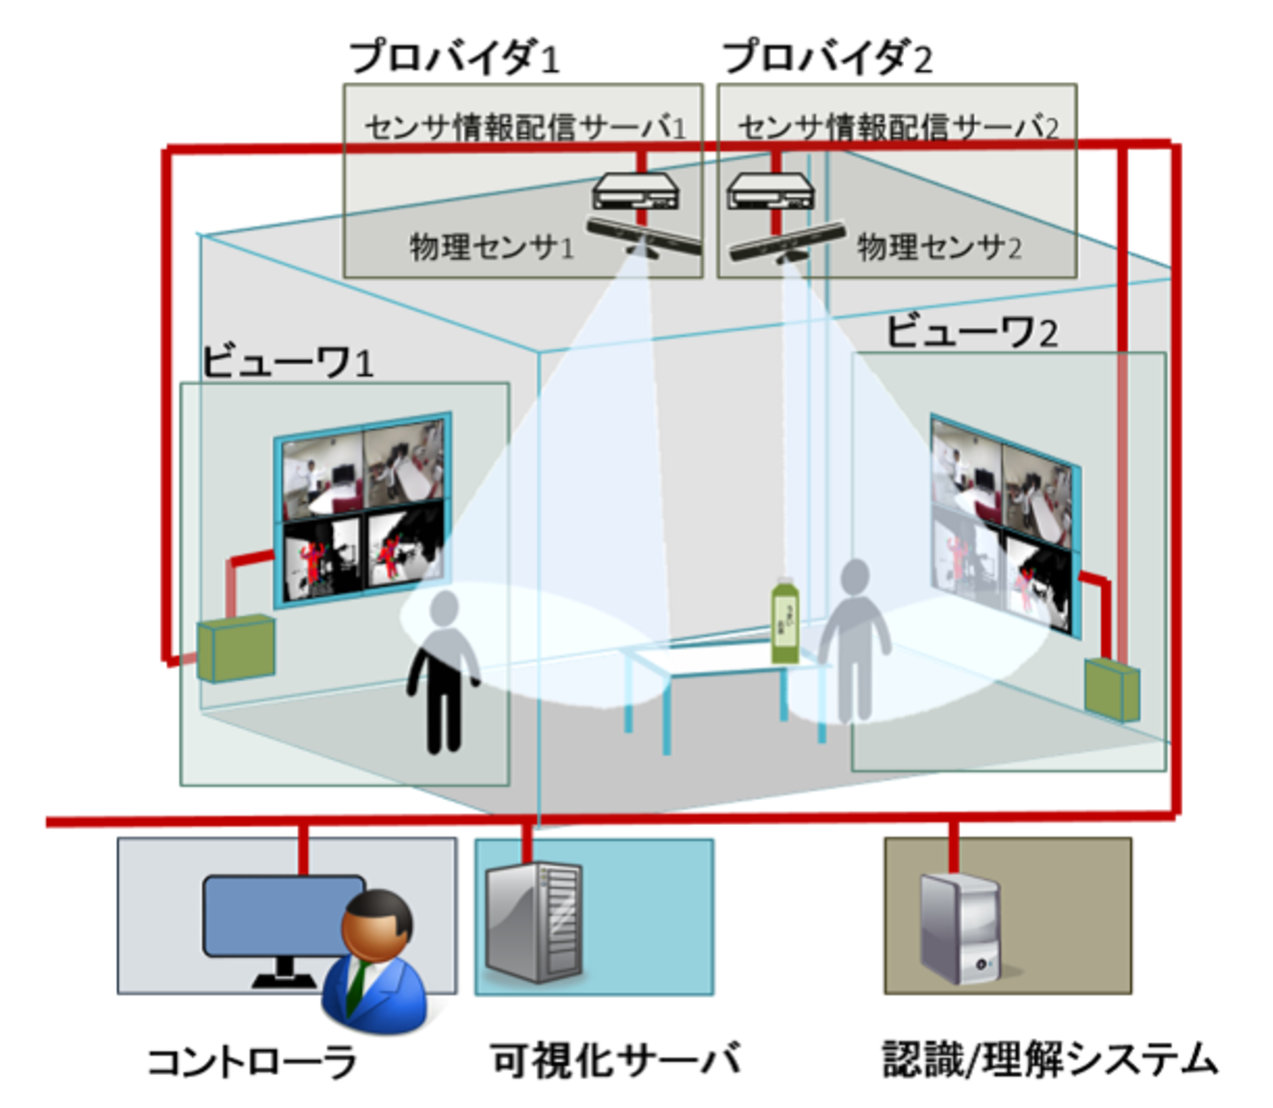
\includegraphics[width=\textwidth,clip]{img/infra.eps}
		\caption{ネットワーク指向型センサ/ディスプレイ基盤}
		\label{fig:infra}
        \end{minipage}%
	\begin{minipage}[b]{0.5\linewidth}
		\includegraphics[width=0.9\textwidth,clip]{img/viewer.eps}
		\caption{複数センサからの情報の閲覧}
		\label{fig:infra}
        \end{minipage}
\end{figure}

この他に, 我々のグループでは階層型イベント検知の仕組みを取り入れ, 低次のイベント情報から高次のイベントを検出するシステムの研究開発を行っている. 
\begin{figure}[h!]
	\centering
	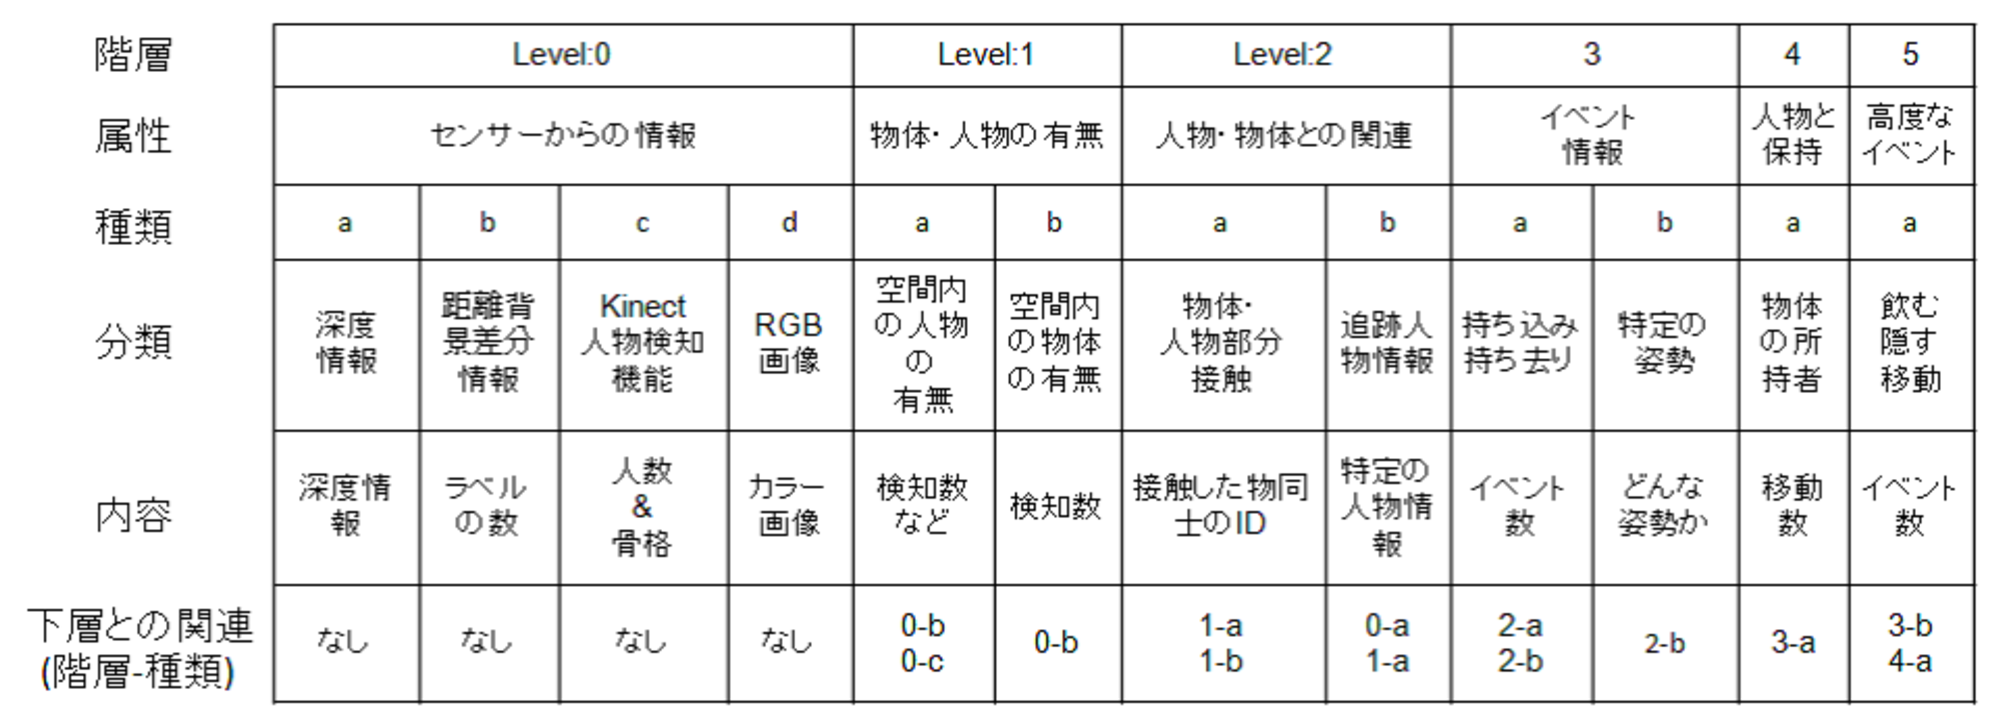
\includegraphics[width=0.47\textwidth,clip]{img/hierarchicalDetection.eps}
	\caption{階層型イベント検知手法}
	\label{fig:hierarchical_event_detecion}
\end{figure}

室内シーン内で起こるイベントの種類は無数あり, 検知したいイベント数が増えてくるとヒューリスティックにイベントを検知する従来のシステムでは困難となってくる. 
